\documentclass{article}
\usepackage{graphicx}
\usepackage{amsmath}
\usepackage[margin=0.8in]{geometry} % Set custom margin size

\title{Assignment 4 Report}
\author{Muhammad Rehan}
\date{April 28, 2024}

\begin{document}
\maketitle

\section*{Introduction}
This report summarizes the development and testing of my Python program to calculate areas under curves using Monte Carlo estimation and numerical integration. The assignment required me to do the following tasks for each question: plotting the function, calculating Monte Carlo estimates, deriving mean and standard deviation, performing integration, and computing percentage error.

\section*{Methodology}
The program includes functions for plotting, Monte Carlo estimation, and integration. The primary functions are:
\begin{itemize}
    \item \texttt{plot\_function}: Plots the given function over a specified range, with an option to save the plot.
    \item \texttt{monte\_carlo\_area}: Estimates the area under a curve using the Monte Carlo method.
    \item \texttt{monte\_carlo\_stats}: Calculates the mean and standard deviation of Monte Carlo estimates.
    \item \texttt{calculate\_integral}: Uses numerical integration to find the area under a curve.
    \item \texttt{percentage\_error}: Computes the percentage error between analytical integration and Monte Carlo estimation.
\end{itemize}

\section*{Implementation}
The program applies the functions to three questions, each with a unique mathematical expression:
\begin{enumerate}
    \item \(f(x) = \sqrt{\sin^2(x) + 1}\), from \(x = 0\) to \(x = 2\).
    \item \(f(x) = x^3\), from \(x = 2\) to \(x = 3\).
    \item \(f(x) = \cos(x^2)\), from \(x = 2\) to \(x = 3\).
\end{enumerate}

Each question includes plotting the function, estimating the Monte Carlo mean and standard deviation, integrating, and calculating the percentage error. The plots are saved to files for further analysis.

\section*{Results}
The program's output includes the Monte Carlo mean, standard deviation, integrated result, and percentage error for each question. These results are consistent with the expected outcomes, indicating that the Monte Carlo method provides an accurate estimate of the area under each curve.


\section*{Figures}

\begin{figure}[htbp]
    \centering
    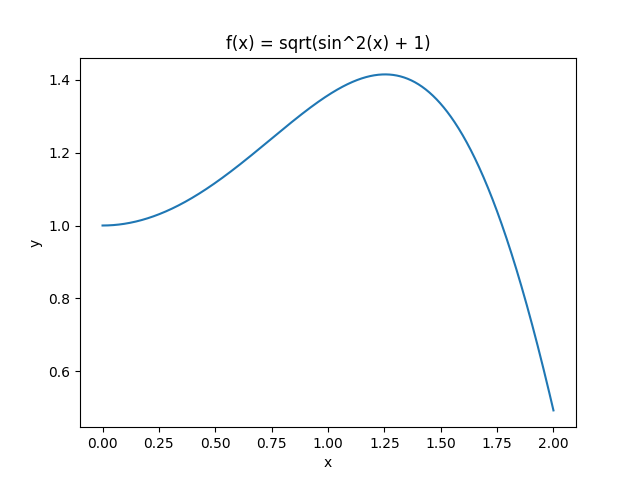
\includegraphics[width=0.5\linewidth]{plot1.png} % Adjust width of the figure
    \caption{Plot of \(f(x) = \sqrt{\sin^2(x) + 1}\).}
\end{figure}

\begin{figure}[htbp]
    \centering
    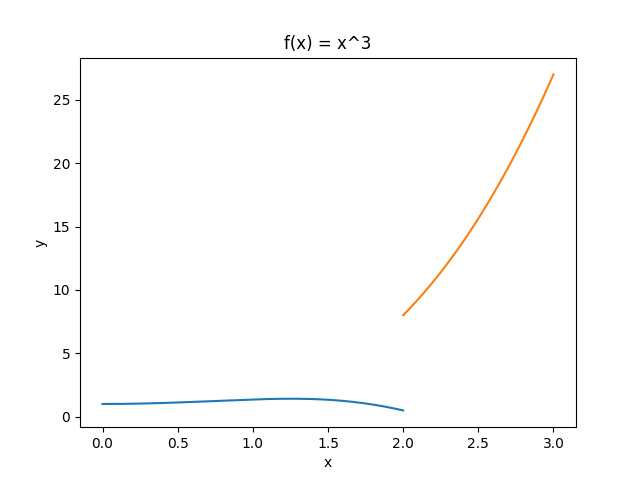
\includegraphics[width=0.5\linewidth]{plot2.png} % Adjust width of the figure
    \caption{Plot of \(f(x) = x^3\).}
\end{figure}

\begin{figure}[htbp]
    \centering
    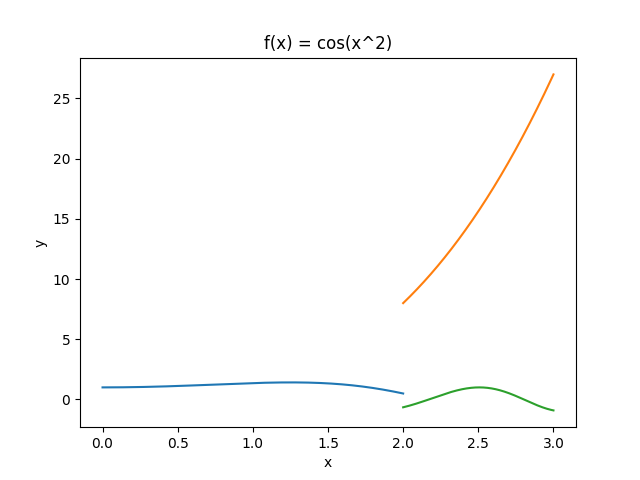
\includegraphics[width=0.5\linewidth]{plot3.png} % Adjust width of the figure
    \caption{Plot of \(f(x) = \cos(x^2)\).}
\end{figure}

\end{document}

